\documentclass[OPS,authoryear,toc]{lsstdoc}
% GENERATED FILE -- edit this in the Makefile
\newcommand{\lsstDocType}{RTN}
\newcommand{\lsstDocNum}{063}
\newcommand{\vcsRevision}{ec4d71a-dirty}
\newcommand{\vcsDate}{2023-08-18}


% Package imports go here.

% Local commands go here.

%If you want glossaries
%\input{aglossary.tex}
%\makeglossaries

\title{HSC PDR2 Reprocessing and Operations Rehearsal for DRP}

% Optional subtitle
% \setDocSubtitle{A subtitle}

\author{%
Yusra~AlSayyad, 
Jennifer~Adelman-McCarthy, 
Brian~Yanny, 
Orion~Eiger, 
Eric~Charles, 
Sierra~Villarreal, 
Zhaoyu~Yang, 
Wen~Guan, 
Jim~Bosch, 
Colin~Slater, 
Michelle~Gower, 
Tim~Jenness, 
Lauren~MacArthur, 
Eli~Rykoff
}

\setDocRef{RTN-063}
\setDocUpstreamLocation{\url{https://github.com/lsst/rtn-063}}

\date{\vcsDate}

% Optional: name of the document's curator
% \setDocCurator{The Curator of this Document}

\setDocAbstract{%
In 2023, the campaign management team processed 100s of sq degrees of precursor data though a data release production on the new US data facility at SLAC.  This activity demonstrated the production of a data release under simulated operational conditions. 
}

% Change history defined here.
% Order: oldest first.
% Fields: VERSION, DATE, DESCRIPTION, OWNER NAME.
% See LPM-51 for version number policy.
\setDocChangeRecord{%
  \addtohist{1}{YYYY-MM-DD}{Unreleased.}{Yusra AlSayyad}
}


\begin{document}

% Create the title page.
\maketitle
% Frequently for a technote we do not want a title page  uncomment this to remove the title page and changelog.
% use \mkshorttitle to remove the extra pages

% ADD CONTENT HERE
% You can also use the \input command to include several content files.
\section{Introduction}\label{sec:intro}

\subsection{Testing 3\% of a DRP using HSC PDR2}

In preparation for annual DRP (Data Release Processing) campaigns, 
a set of some 17K exposures from the HSC PDR2 dataset were pushed through
a current version of the DRP pipelines.

These exposures are then coadded into 710 tracts, including about 671
WIDE tracts of repeated depth a few in grizy bands, and 39 DEEP+UDEEP 
tracts with up to 426 overlapping exposures in some bands in some UDEEP tracts.
The DEEP+UDEEP tracts covered about 100 square degrees in area, while the
WIDE tracts covered about 1000 square degree to varying depth.

These 17K exposures along with the coadd tracts and other
outputs generated, represent approximately 3\% of the first 
years' Rubin planned DR1 dataset in volume and filecount.

\begin{figure}[h]
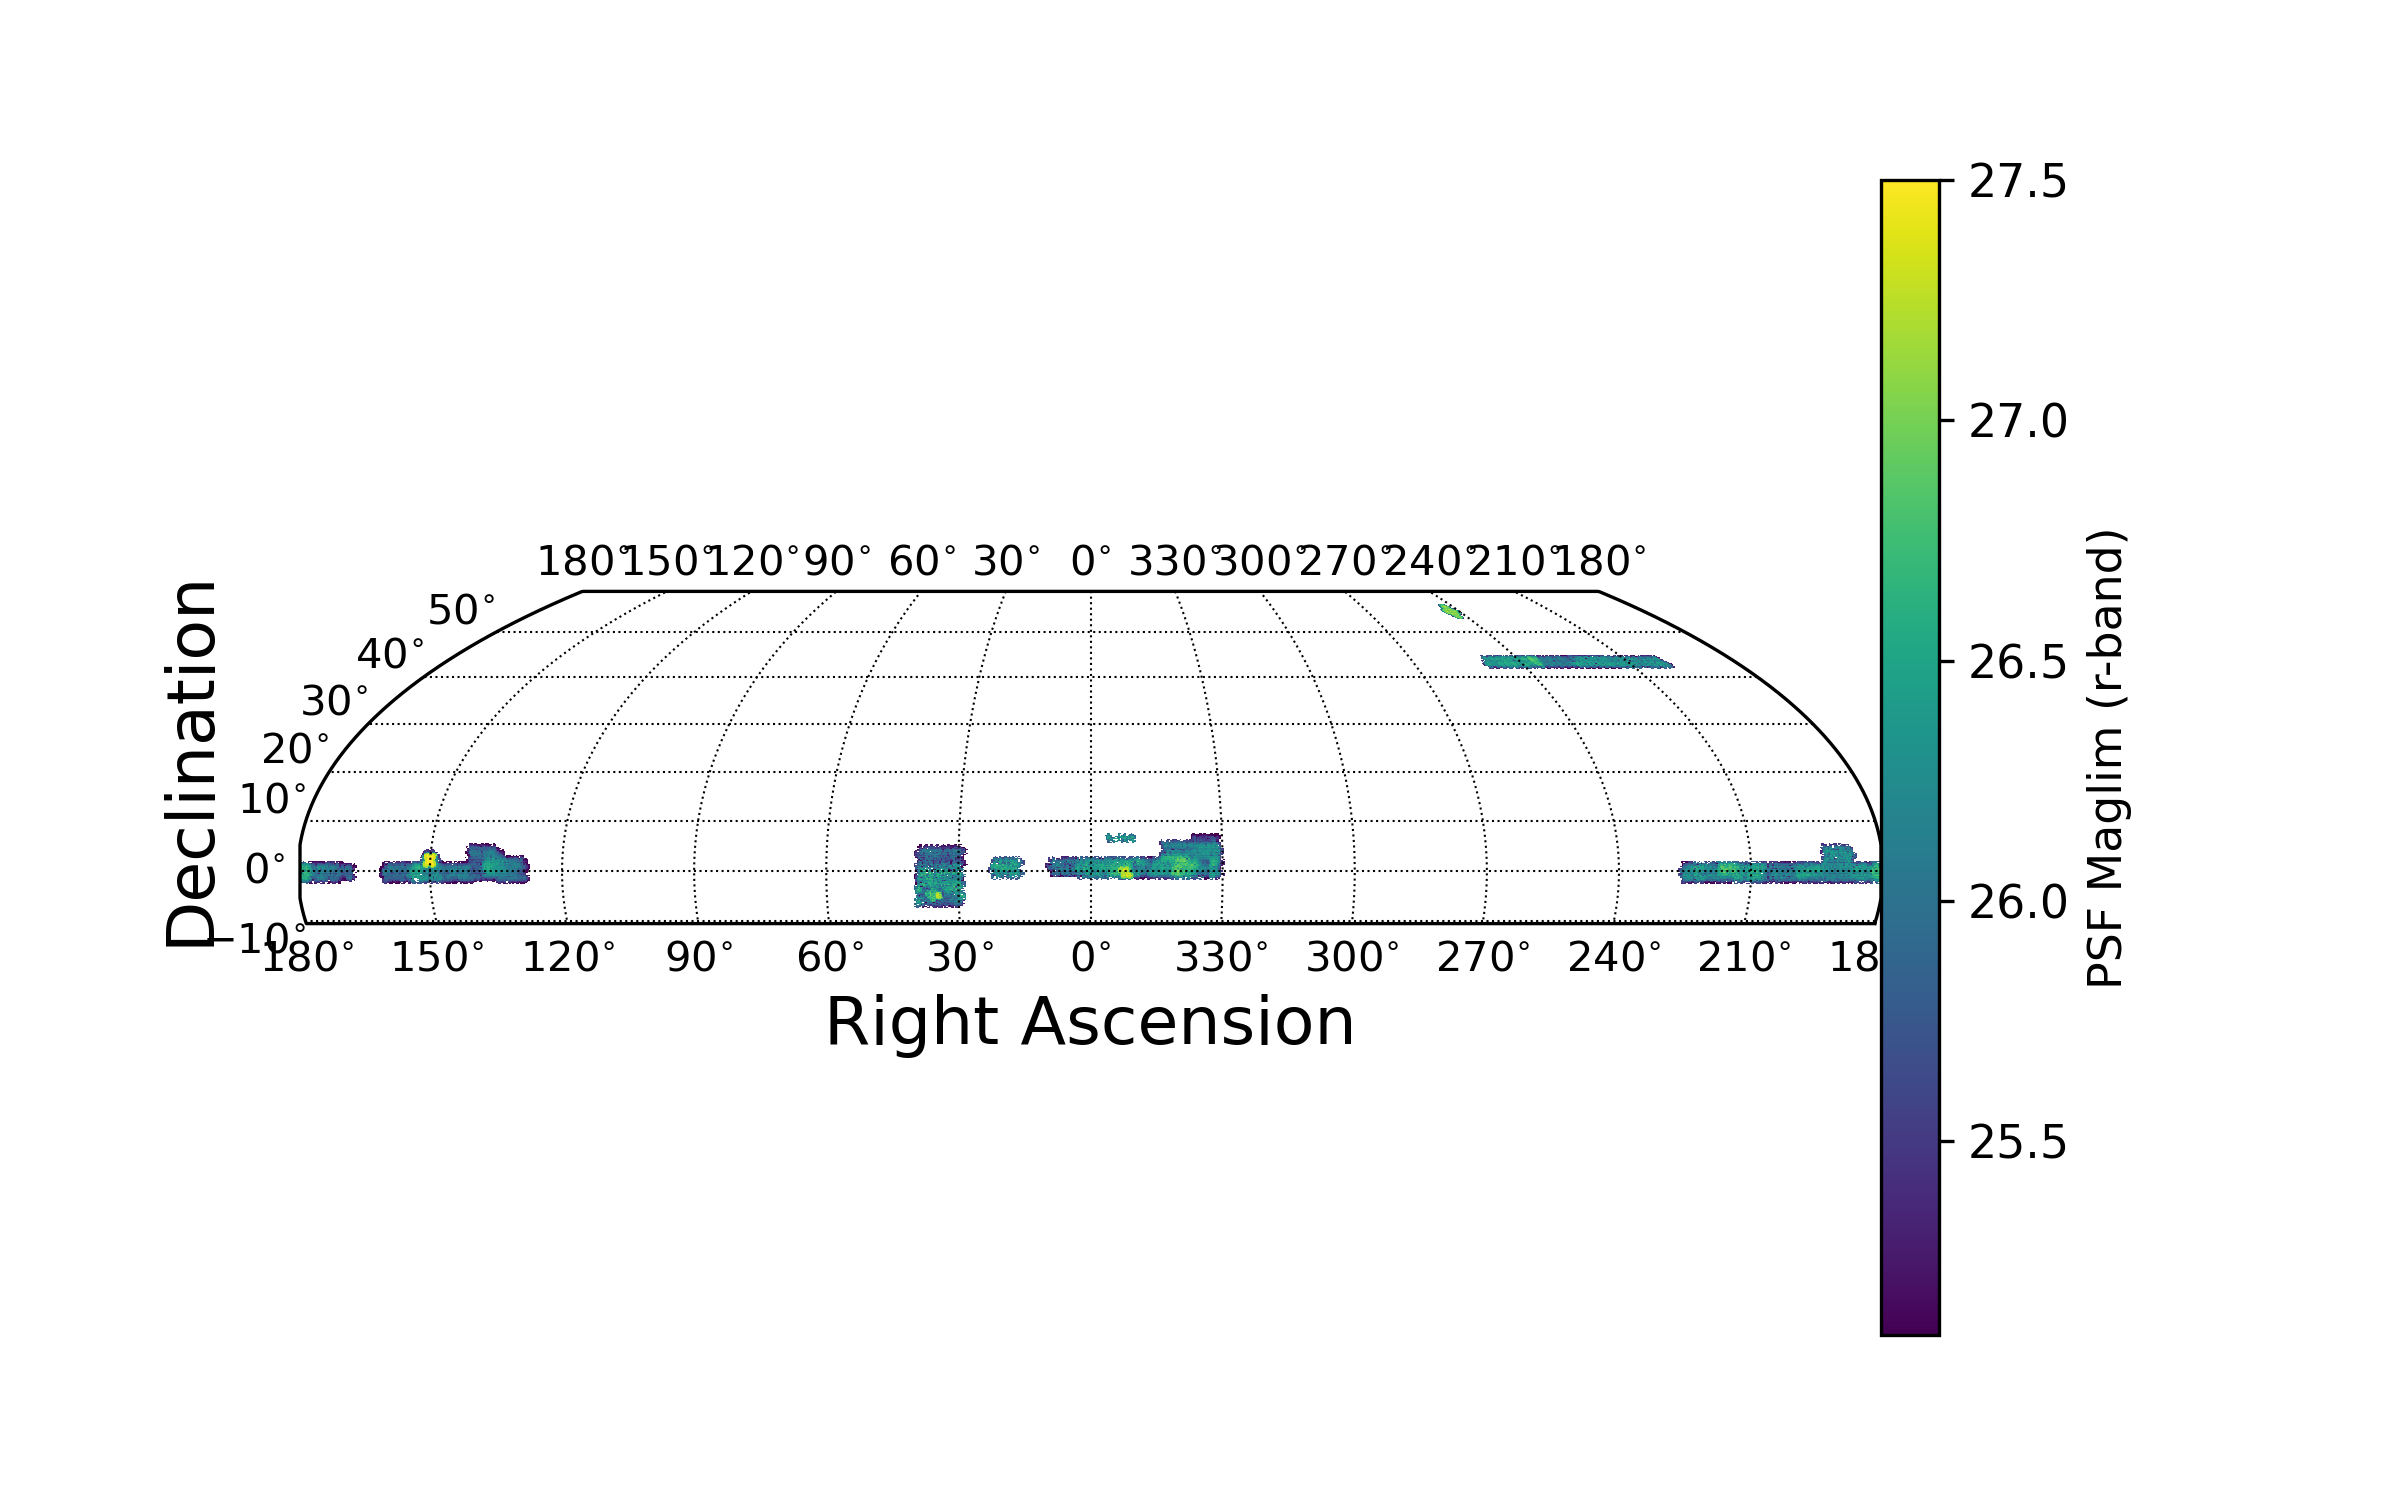
\includegraphics[width=0.9\textwidth]{r_maglim_pdr2.png}
	 \caption{Footprint of PDR2 processed dataset in equatorial coordinates.  \label{fig:footprint1}}
\end{figure}

 \begin{figure}[h]
 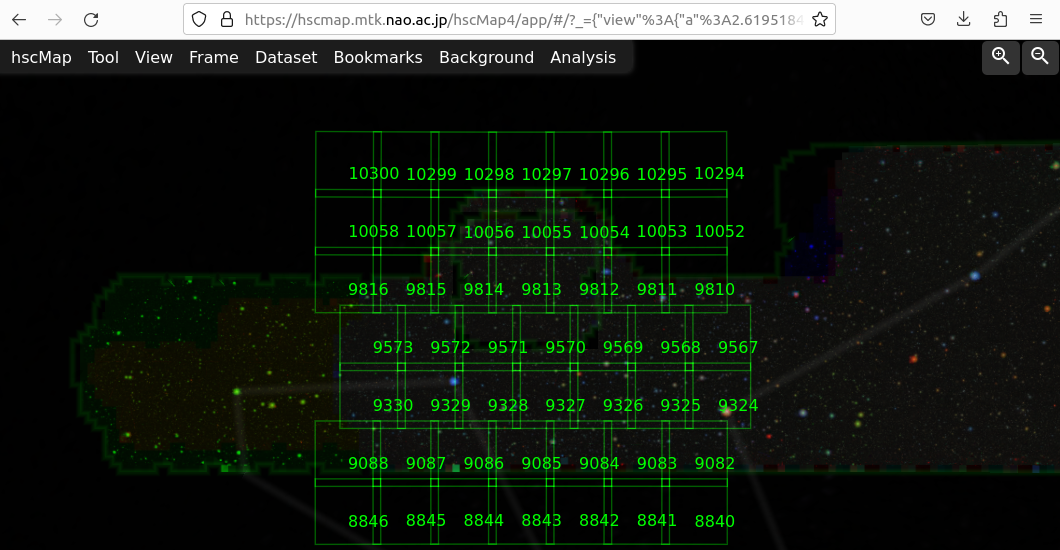
\includegraphics[width=0.9\textwidth]{hscmaptractcosmos.png}
	 \caption{PDR2 close up near COSMOS region (centered near $\rm (RA,DEC) = (150, 2)$ degrees), with tract numbers overlaid.  \label{fig:hscmaptract}}
 \end{figure}

\subsection{PDR processing and instruments: HSC vs. LSSTCam}

Each detector is a 2K x 4K pixel CCD image, of size about 57MB.
There are 103 science quality CCDs/exposure.  Detector 9 is masked due
to known quality issues and ccds 104-112 are not on-sky science chips in
the HSC mosaic.

The HSC sky is divided into 'tracts' and each tract is subdivided 
into 'patches', as defined by the skymap (hsc\_rings\_v1) which maps 
tract number to a square region in (RA,DEC) coordinates.

For HSC, each tract covers about 2.7 sq degrees on the sky and is
subdivided into 81 patches on a $9 \times 9$ grid.

In contrast, the full LSSTCam has 4K x 4K pixel CCDs, there are 
189 science CCDs each about 100 MB in size.  Furthermore each tract 
on the sky is divided into a $7\times 7$ grid of patches.

For purposes of this exercise, the calibration exposures (
flat fields in each band, biases, non-linearity maps, sky pupil per 
band, bad pixel, bad column,  gain and full well levels per amplifier) are 
all taken as given 'ancillary' inputs, pre-constructed and outside the
scope of this campaign.

For DP1, DP2 and DR1 all good visits obtained to over a certain time
interval, six months to one year in length are gathered at the
start of a DRP.  All raw exposures are processed through 
step1 (which consists of pipetasks for Instrument Signature 
Reduction (ISR), image and PSF characterization, source detection 
and measurement), 
step2a (combine gather source tables), and step2b (perform 
astrometric calibration with a 2MASS or eventually Gaia reference catalog,
extract calibration star catalogs) 
at multiple processing sites if available.  Each visit or detector may 
be processed independently (and many in parallel) 
for steps 1, 2a and 2b.

For the PDR2 HSC exercise, multi-site processing was not yet up, 
and so all processing was done at one site (the USDF at SLAC).

Following step2b, the extracted, (and relatively small),
calibration star catalogs are gathered together over the entire campaign
footprint and are used in step2c to generate a single Forward 
Global Calibration Module (FGCM) photometric solution with zeropoints for
each exposure processed.

These astrometric solutions and photometric zeropoints from steps 2b and 2c
respectively are applied in step2d and gathered together by visit in step2e.

There may be (and in the case of PDR2 there was) a 'visit-veto list' of 
poor quality (i.e. bad seeing) exposures identified at the end of step2e but 
prior to the start of step3.  A subcollection is made containing only 
the remaining good visits, which are used for further processing.  

For the HSC PDR2 case, about 2.5K out of 17.3K visits were rejected 
leaving about 15K visits to be coadded.

Step3 of PDR processing performs coaddition, combining all calibrated 
visit images, first 'warping' them using the astrometric solution to put 
them onto a common geometric footprint and then coadding them weighted 
appropriately by photometric flux zeropoint and noise properties.

The astrometric algorithm used for PDR2 HSC is called 'jointcal'.  This
older algorithm may be replaced by 'gbdes' in future processings, as that
algorithm accounts for 'tree rings', DCR 
(Differential Chromatic Refraction) and other subtle distortions \jira{DM-39933}.

Coadds for the HSC PDR2 footprint are currently done patch-by-patch,
though future processings will also produce 'overlapping cell-based' 
coadds \jira{DM-32345} which further subdivides patches and tracts into regions of 
the sky where the PSF in each band is well-modeled as constant 
across an entire cell with no discontinuous jumps due to detector edges.
These cell-based coadds in turn will allow for the accurate measurement of 
weak lensing shears of all source stacked objects when combined with
a PIFF PSF model.

Between May 2023 and (approx) Sep 2023 the HSC PDR2 was reprocessed with 
Rubin Science pipelines stack version v24.1.0, which was 
based on a weekly stack w\_2023\_11.  Some modifications or fixes 
to the stack were applied during the processing, as described below.

In the sections that follow, we discuss campaign 
management \secref{sec:management}, 
processing \secref{sec:processing} and quality 
assurance \secref{sec:qa} details of the HSC PDR2 campaign.

%5\begin{itemize}
%\item Campaign Management and communication is discussed in \secref{sec:management}
%\item An overview of the processing is given in \secref{sec:processing}
%\item Quality assurance and feedback to processing is discussed in  \secref{sec:qa}
%\end{itemize}


\section{Campaign Management and Communication} \label{sec:management}

Here we cover the management structures in place for HSC PDR2 
this includes the groups and meetings like the change control for 
the pipeline version.

\subsection{Oversight}

Science Pipelines, DM Middleware, Campaign Management (CM), and Data Production
were all involved in HSC PDR2 production.

\subsection{Data Production}

For HSC PDR2, the active membership of the team was:
\begin{itemize}
\item Yusra AlSayyad -- Lead
\item Jennifer Adelman-McCarthy Pilot
\item Brian Yanny co-Pilot
\end{itemize}


\subsection{Campaign Management}
\begin{itemize}
\item Eric Charles -- Lead
\item Orion Eiger
\item Sierra Villarreal
\item Fritz Mueller
\end{itemize}

\subsection{System Performance}
\begin{itemize}
\item Colin Slater - Lead Verification and Validation Scientist
\end{itemize}

\subsection{Coordination}

The Data Production Lead defines campaigns (input datasets, software stack version, set of
steps (of pipetasks) to run, and rough deadline) to be run 
here \url{https://confluence.lsstcorp.org/display/DM/Campaigns}, and assigns pilots and co-pilots.
For the HSC PDR2 campaign, overall notes are kept here: \url{https://confluence.lsstcorp.org/display/DM/2023+Internal+HSC+PDR2+Reprocessing+at+the+USDF}.   As this dataset has been previously processed, it was useful
to reference the earlier reprocessing from 2020 to compare visit lists, tract lists and other notes:
\url{https://confluence.lsstcorp.org/display/DM/S20+HSC+PDR2+Reprocessing}.

During the production of HSC PDR2 weekly coordination meetings were held with the Data Production 
and V\&V leads, the pilots, PanDA experts, and Middleware and CM developer reps. 

\subsection{Work Management}

We used Jira to track work related to the HSC PDR2 campaign.
%Epics and milestones were created in the \texttt{DM} Jira Project.
The main ticket was \jira{DM-39132} with subtickets for each step.
These tickets contained processing notes, and special situations that came up.

The slack channel {\it\#ops-cm-team} was used for questions and discussion as issues arose.
The channel {\it\#dm-hsc-reprocessing} was also a valuable resource as weekly processing of small
sets of HSC data were discussed here.

\subsection{Change Control Decisions during processing}

The Science Pipelines team working with V\&V and middleware determined which weekly release to use as a base
software distribution for the v24 stack.  Some tickets subsequent to the initial v24 stack branching
were backported into the v24 branch.  PDR2 used v24.1.0.rc2 for steps 1, 2a and 2b.

During processing, the Science Pipelines team continued to monitor progress and determine if updates were
needed to the software while processing.

The stack was updated to v24.1.0.rc3 for step 2c and beyond to incorporate an updated fgcm (photometric
calibration map covering the whole HSC PDR2 footprint) \jira{DM-39342}.

During the Running of step3 and step7 two hot fixes were incorporated into processing, making use
of the CM '$\rm custom\_lsst\_setup$' feature, which allowed a github branch of code, along with a EUPS setup
file, to be loaded for processing on top of the base v24.1.0.rc3 stack.

The first hot fix was to the $\rm meas\_algorithms$ module to enable more robust dynamic sky estimation in very
crowded fields -- without this fix, large sections of the UDEEP tracts simply had no good detections or
measurements due to lack of sky objects.

The second hot fix was to the healSparse module to enable healSparsePropertyMaps (a step3 pipetask) and 
consolidateHealSparsePropertyMaps (step7) to proceed in cases where a tract or patch was not complete.
This allowed the NSC PDR2 production to proceed even for tracts which were not completely filled in.

We note that it was determined here that the stack and all hotfixes used to generate the quantum graph
needs to be identical to the stack used to process the quantum graph.  That is the setup used to make the graph
needs to have all the pieces used to execute the graph otherwise hotfix code patches will not work.

\subsection{Production Hardware and Workflow software system}

Panda Doma Queues, one may view the number of jobs currently running in each queue here:
\url{https://panda-doma.cern.ch/dash/region} (auth required, increase Show entries from 20 to 50)
A Pull mode queue means there is a pilot job running on a worker node which pulls jobs to it from PanDA and
can handle large numbers of jobs per pilot.  A Push mode queue means that there is only one pilot per
job (usually for very long running or high memory jobs). 

\normalsize 
\begin{center}
\begin{longtable}{|l|r|r|r|r|l|} 
\caption{PanDA Queue Names, Sizes, Time limits} \label{tab:pandaqueues}\\
\hline 
\textbf{Name}&\textbf{Slots}&\textbf{Memory}&\textbf{Wallclock}&\textbf{Push/Pull}&\textbf{Notes} \\ 
\hline
$\rm SLAC\_Rubin\_Merge$ & 200 & $<16$ GB & 24h & Push & MergeExecutionButler \\
$\rm SLAC\_Rubin$ & 4000 & $<4$ GB & 24h & Pull & 600 jobs/pilot \\
$\rm SLAC\_Rubin\_Medium$ & 3000 & $4-8$ GB & 24h & Pull &  600 jobs/pilot\\
$\rm SLAC\_Rubin\_Himem$ & 2500& $8-18$ GB & 24h & Pull &  600 jobs/pilot \\
$\rm SLAC\_Rubin\_Extra\_Himem$ & 1500 & $>18$ GB & 96h & Push & 1 job/pilot \\
\hline
\end{longtable} 
\end{center}
\normalsize


\section{PDR2 processing on USDF cluster} \label{sec:processing}

The data processing was done using the Production and Distributed Analysis System (PanDA; \citeds{DMTN-168}) at the USDF at SLAC.
The PanDA system handled workflow orchestration and job retries.
Based on pre-production testing, five PanDA queues (\texttt{lowmem}, \texttt{mediummem}, \texttt{highmem}, \texttt{extra-highmem}, and  \texttt{merge}) were deployed. Each queue had fixed numbers of slots, memory limits, wallclock runtime limits and pull-or-push mode as described in this table:

The production processing was organized into seven logical ``steps''.
The high level workflow of workflows and the step organization is described in \citeds{RTN-001} Sect. 2.1.4.
Pipelines, V\&V, and Processing teams all focused on one step at a time.
Before the production processing started in each step, ``pilot runs'' with candidate software were carried out and signed off by V\&V and Pipelines teams
(Sect \ref{sec:management}).

The workflow generation and submission were done via the PanDA BPS plugin a terminal window logged into the USDF.
The BPS YAML configurations can be found in a branch of the  GitHub repo (https://github.com/lsst-dm/cm-prod).

Workflow progress was tracked via PanDA's iDDS monitoring page deployed at CERN and the JIRA-based campaign tooling (\citeds{RTN-023}).

On many occasions (20\%) rescue workflows skipping successful jobs were run.

The processing took place  between May 2023 to Sep 2023 and the total cpu usage over the course of PDR2 was approximately XXXX M core-hour; the compute resource usage is summarized below.
Notable issues which came up during the production were summarized as follows.

The Campain Management tools: cm_prod and cm_tools : https://github.com/lsst-dm/cm_prod were used to help manage this production.  

A summary of errors for all steps can be found at : https://confluence.lsstcorp.org/pages/viewpage.action?pageId=222728293

\begin{itemize}

\item Step1
\begin{itemize}

  \item
Step one was run using version v24.1.0.rc2 of the lsst software stack. We ran it in three distinct pieces, all with their own cm database.  WIDE: 14473 exposures (note exposure 428 (y-band) from the 2020 processing, left out accidentlly). DEEP: 1832 exposure. UDEEP: 1010 exposures (up to 426  exposures in one band covering a single tract on the sky: tract 9813, z-band).
  \item

17315 exposures divided into 39 groups for processing with PanDA/slurm workload/workflow/batch system on 3,000 cores at USDF typically took 2.5 hours to generate quantum graph + EXEC butler per group run time typically 2 hours (not counting long tail), when clustering of 5 pipetasks of step1 in place. Long tails, timeout, hangs from processing extended run time to a couple weeks wallclock for all of step1.

Processing runs in 4GB/core requestMemory allocation.


\end{itemize} %step1

\item Step2
\begin{itemize}

 \item
Step 2 was broken down into 

\end{itemize} %step2

\item Step3
\begin{itemize}

  \item
  Large numbers of simultaneous assembleCoadd (= image coaddition) jobs led to ``too many request'' errors reading from the object store (\jira{PREOPS-1034}).
  Algorithmically, the rate spike was because the coaddition was done in small chunks and data reading happened for each chunk and each input warp.
  This could be alleviated by caching input files instead of requesting them from the object store each time.
  The caching configuration in the butler repo was changed so not to expire anything in coaddition.
  The first 7 step3 workflows needed to be redone due to this problem.
  This also led to the investigation of the ``hidden'' errors in the coadds, where coadd images were reported ok but actually had problems (\jira{DM-33786}).
  More details are discussed in Sect. \ref{sec:qa}).
  Later we found out that the initial fix of the caching was too aggressive and led to out-of-disk-space errors for a couple of large faro tasks (matchCatalogsPatchMultiBand and matchCatalogsTract), but subsequently caching was better optimized to be sufficient for coadds, but not so much to cause disk space problems for the faro tasks.

  \item
  Long-running forcedPhotCoadd jobs were failing/re-attempting at a much higher rate than before, caused by a change in the PanDA pilot version, which reset the job heartbeat timeout limit back to its default of 2 hours, whereas it had been set to 20 hours previously.
  This issue also uncovered the need for more frequent heartbeat message logging for long-running forcedPhotCoadd (\jira{DM-33854}) and faro tasks (\jira{DM-33820}).
  The timeout limit was set again to 20 hours to allow step3 production to continue efficiently.

  \item
  About once every two workflows or so, a deblend job or two failed due to out-of-memory error (\jira{DM-33690}), because of very bright/large objects on the coadd image.
  These failures were fixed in rescue workflows, but required long run times ($>$10 hrs) and large memory ($\approx$~40 GB) using the \texttt{extra-highmem} queue, though ultimately with deblending results that were likely unreliable.
  The most extreme example (tract 4648, patch 29) took 12 unsuccessful attempts before finally succeeding in the \texttt{extra-highmem-non-preempt} queue (\jira{DM-33947}), after 2 days 22.7 hours run time, 190 GB memory, and extra efforts from the PanDA team to bypass heartbeat logging issues.
  This was the last image processing job to be completed in step3.
  \jira{DM-33690} implemented deblending configuration changes to skip these problematic deblends, so this should not be an issue subsequent to DP0.2.

  \item
  The large faro tasks matchCatalogsPatchMultiBand and especially matchCatalogsTract took long run times and large memory ($\approx$~130 GB for the latter).
  They needed to be run on the \texttt{extra-highmem} queue and were also prone to preemption and multiple re-attempts due to heartbeat logging issues (\jira{DM-33820)}.

 \item
  Some delays arose when jobs became stuck as they were unexpectedly scheduled to a non-IDF queue, which had its ``region'' set erroneously to ``LSST'', same as for the IDF queues.
  This issue was corrected by the PanDA support team.

  \item
  There were also some delays due to unexpected consequences from PanDA server and client updates, again resolved by the PanDA support team.

\end{itemize} %step3

\item Step4
\begin{itemize}

  \item
  An attempt was made to use the Google Artifact Registry (GAR) instead of Docker Hub to download the LSST processing stack.
  However, this resulted in intermittent authentication problems that led to 20-50\% job failures in three step4 workflows.
  Despite an attempt to reconfigure the IDF computing cluster involved, the authentication problems continued, and we reverted to using Docker Hub and reran the affected workflows.

  \item
  We also saw a drop in the maximum number of running jobs in the IDF queue involved, from nearly 4000 down to as few as about 2000, possibly related to the above authentication issues.
  PanDA support increased the maximum number of new worker nodes created from
50 to 80 to help stabilize the number of running jobs back to nearly 4000.


\end{itemize} %step4

\item step5
\begin{itemize}

  \item
  We encountered a very slow start to jobs running on the PanDA system due to the large number of jobs per task ($>$100,000) in the first step5 workflow.
  This was solved by reducing the maximum number of jobs per task from the default value of 70,000 down to 30,000, so that a single large task was divided into smaller ``chunks'' (each with $<$30,000 jobs) that ran much more efficiently in the PanDA system.
We do need an  iDDS server with more resources.

\end{itemize} %step5

\item step6, step7
\begin{itemize}

  \item Minor or no issues.

\end{itemize} %step6,7

\end{itemize} %all steps

 \begin{figure}
 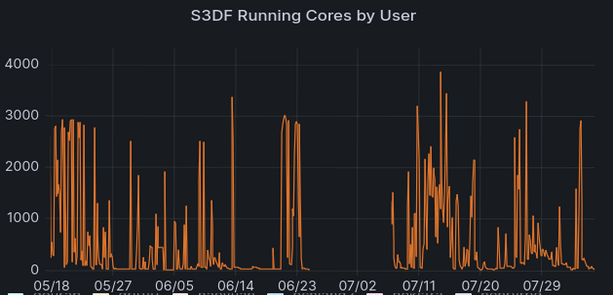
\includegraphics[width=0.9\textwidth]{Campcorespdr2.png}
         \caption{Cores in use in PDR2 step1,step2,step3 campaign.}  \label{fig:campaigncores}
 \end{figure}




\section{Data Product Quality Assurance} \label{sec:qa}

During PDR2, the Verification and Validation Team was responsible for identifying problems and bugs
in the pipelines and data products. There were there main phases of V\&V work:

\begin{itemize}
\item A period of analysis using a “pilot run” before the start of production, which ran a single
tract through all steps of the pipeline, using the codebase planned for the release.
\item Two “gates”, one at the end of single frame processing and another after coadd construction,
where production was halted for V\&V to confirm that all the data products were ready before moving
on to the next step of processing.
\item Spot checks during processing, and follow-up of unexpected errors or failed tasks.
\end{itemize}

During these main phases, the V\&V team made extensive use of the plotting capabilities in
analysis\_drp along with adding new diagnostic plots. Much of the analysis was performed by writing
notebooks to test out new diagnostics for data products that were recently added to the pipelines.
The team also drew on experience from many prior processings (particularly of Hypersuprime-cam) to
quickly distinguish ``known'' problems from new problems.

A notable success occurred during coadd construction, when as part of the spot checks during
processing the team noticed some regions inside successfully-processed patches had no coadd sources
detected. One of the plots that lead to this discovery is shown below. This was particularly
unexpected because entire patches are expected to succeed or fail entirely, it was highly unusual
for portions to fail silently.

The eventual explanation was that the coaddition code operated on sub-patch-sized regions
sequentially, in order to limit peak memory usage, and so it would read from disk different portions
of the input warp images as it progressed. On a typical POSIX filesystem these reads typically
either all succeed or all fail, but in the cloud environment the object store would sometimes deny
individual requests as a form of rate-limiting. The coaddition code could have caught this, but
since that type of failure was never encountered in prior usage, it mistakenly proceeded without
raising an exception. Because this issue was identified early during coaddition, only a few days
worth of processing had to be redone.

% \begin{figure}
% \includegraphics[width=0.7\textwidth]{coadd_bug.png}
% \caption{The regions of the coadd that lack any Objects were caused by an unexpected failure mode in
    % accessing the input images, which was possible on cloud infrastructure but not seen on POSIX
    % files. \label{fig:coadd}}
% \end{figure}

The data previews are also a chance to learn from the issues that we didn’t catch during V\&V; most
notably were two cases where invalid flux calibrations were being applied to certain measurement
algorithms, resulting in NaNs in the output. This case shows the value of having a wide breadth of
testing coverage. For future releases we will ensure that we have some form of testing for every
column in every user-facing data product. Even if the tests are relatively simple, they may identify
significant issues.

As one further example of potential issues encountered during production, a few days after the start
of single frame processing the pipelines began to show hundreds of failures with the error message
\texttt{Exception ValueError: No reference objects supplied}. This was not seen in the pilot run, so
production was paused while we investigated. By plotting the locations of these failures on the sky,
we determined that these sensors fell outside the footprint of the stellar input catalog, and hence
there were no stars available for calibrating these images. These were thus “unprocessable” and no
corrective action was required, but it illustrated the value of realtime error collection and
monitoring during production.




\appendix
% Include all the relevant bib files.
% https://lsst-texmf.lsst.io/lsstdoc.html#bibliographies
\section{References} \label{sec:bib}
\renewcommand{\refname}{} % Suppress default Bibliography section
\bibliography{local,lsst,lsst-dm,refs_ads,refs,books}

% Make sure lsst-texmf/bin/generateAcronyms.py is in your path
\section{Acronyms} \label{sec:acronyms}
\addtocounter{table}{-1}
\begin{longtable}{p{0.145\textwidth}p{0.8\textwidth}}\hline
\textbf{Acronym} & \textbf{Description}  \\\hline

2MASS & Two-Micron All Sky Survey \\\hline
BPS & Batch Production Service \\\hline
CCD & Charge-Coupled Device \\\hline
CERN & European Organization for Nuclear Research \\\hline
CM & Configuration Management \\\hline
DCR & Differential Chromatic Refraction \\\hline
DEC & Declination \\\hline
DEEP & Deep Extragalactic Evolutionary Probe \\\hline
DM & Data Management \\\hline
DMTN & DM Technical Note \\\hline
DP1 & Data Preview 1 \\\hline
DP2 & Data Preview 2 \\\hline
DR1 & Data Release 1 \\\hline
DRP & Data Release Production \\\hline
DS9 & Deep Space 9 (specific astronomical data visualisation application; SAOImage) \\\hline
EUPS & Extended Unix Product System \\\hline
FGCM & Forward Global Calibration Model \\\hline
GB & Gigabyte \\\hline
HSC & Hyper Suprime-Cam \\\hline
ISR & Instrument Signal Removal \\\hline
LSST & Legacy Survey of Space and Time (formerly Large Synoptic Survey Telescope) \\\hline
MB & MegaByte \\\hline
NAOJ & National Astronomical Observatory of Japan \\\hline
OPS & Operations \\\hline
PDR & Preliminary Design Review \\\hline
PDR2 & Public Data Release 2 (HSC) \\\hline
POSIX & Portable Operating System Interface \\\hline
PSF & Point Spread Function \\\hline
PanDA &  Production ANd Distributed Analysis system \\\hline
RA & Right Ascension \\\hline
RAM & Random Access Memory \\\hline
RTN & Rubin Technical Note \\\hline
SLAC & SLAC National Accelerator Laboratory \\\hline
UK & United Kingdom \\\hline
US & United States \\\hline
USDF & United States Data Facility \\\hline
VM & Virtual Machine \\\hline
YAML & Yet Another Markup Language \\\hline
bps & bit(s) per second \\\hline
\end{longtable}

% If you want glossary uncomment below -- comment out the two lines above
%\printglossaries





\end{document}
